\section{Optimal Experimental Design Considerations}

In this section we return to the nonlinear examples presented in the previous chapter and address the choices made in experimental design.
By revisiting the examples at the end of the previous chapter, we demonstrate that the decisions made regarding measurement equipment and/or location have an impact on the reduction of uncertainty and accuracy of the MUD point.

We study the impact of more precise measurement devices on the convergence rates for the parameter estimates.
First we return the problem of estimating the rate of exponential decay by incorporating measurements taken in time into the WME map from [TK - ch4 section here].
To complement these results, we show them alongside ones generated with equipment that measures at twice the temporal frequency.

Next, we study the same question of the impact of measurement precision for the PDE problem introduced in [TK - ch4 section here].
A similar complementary problem is solved where information about the sensitivity of measurement locations is used to inform improved placement of a hundred sensors.
In this example, we walk through the sorts of analyses a modeler might conduct in order to select an experimental design through simulation and show a significant improvement in the accuracy of the MUD point.


%%%%%%%%%%%%%%%%%%%%%%%%%%%%%%%%%%%%%%%%%%%%%%%%%%%%%%%%%%%%%%%%%%%%
%%%%%%%%%%%%%%%%%%%%%%%%%%%%%%%%%%%%%%%%%%%%%%%%%%%%%%%%%%%%%%%%%%%%
\subsection{ODE Example Revisited}
%%%%%%%%%%%%%%%%%%%%%%%%%%%%%%%%%%%%%%%%%%%%%%%%%%%%%%%%%%%%%%%%%%%%
\FloatBarrier
%%%%%%%%%%%%%%%%%%%%%%%%%%%%%%%%%%%%%%%%%%%%%%%%%%%%%%%%%%%%%%%%%%%%
\subsubsection{Different Measurement Equipment}

One way by which modelers can improve the quality of parameter estimates is by collecting more data.
We consider what would happen if our measurement equipment were able to capture twice as many observations.
Instead of using equipment that operates at $100$Hz, we take $200$ measurements every second, resulting in 400 equispaced observations for $t \in (1,3)$.
All other choices involved in the experiment (assumed equipment tolerance, number of trials, parameter samples), are kept the same.
We refer to this setup wit faster measurement equipment as the ``alternative'' design.


We show the resulting predictions for the signal using MUD points from twenty repeated trials in Figure~\ref{fig:ode-alt-reference} using the first twenty (middle) and all of the measurements (bottom).
The top of the figure shows the solution from the original setup \ref{fig:ode-reference} for visual comparison.
The true signal is well-recovered even with a small subset of the data collected.
By the time all measurements are used, the stability of the solutions\---with respect to the noise that may have polluted them\---is evidenced by the fact that the red lines representing solutions disappear against the backdrop of the true signal in black.

\begin{figure}[htbp]
  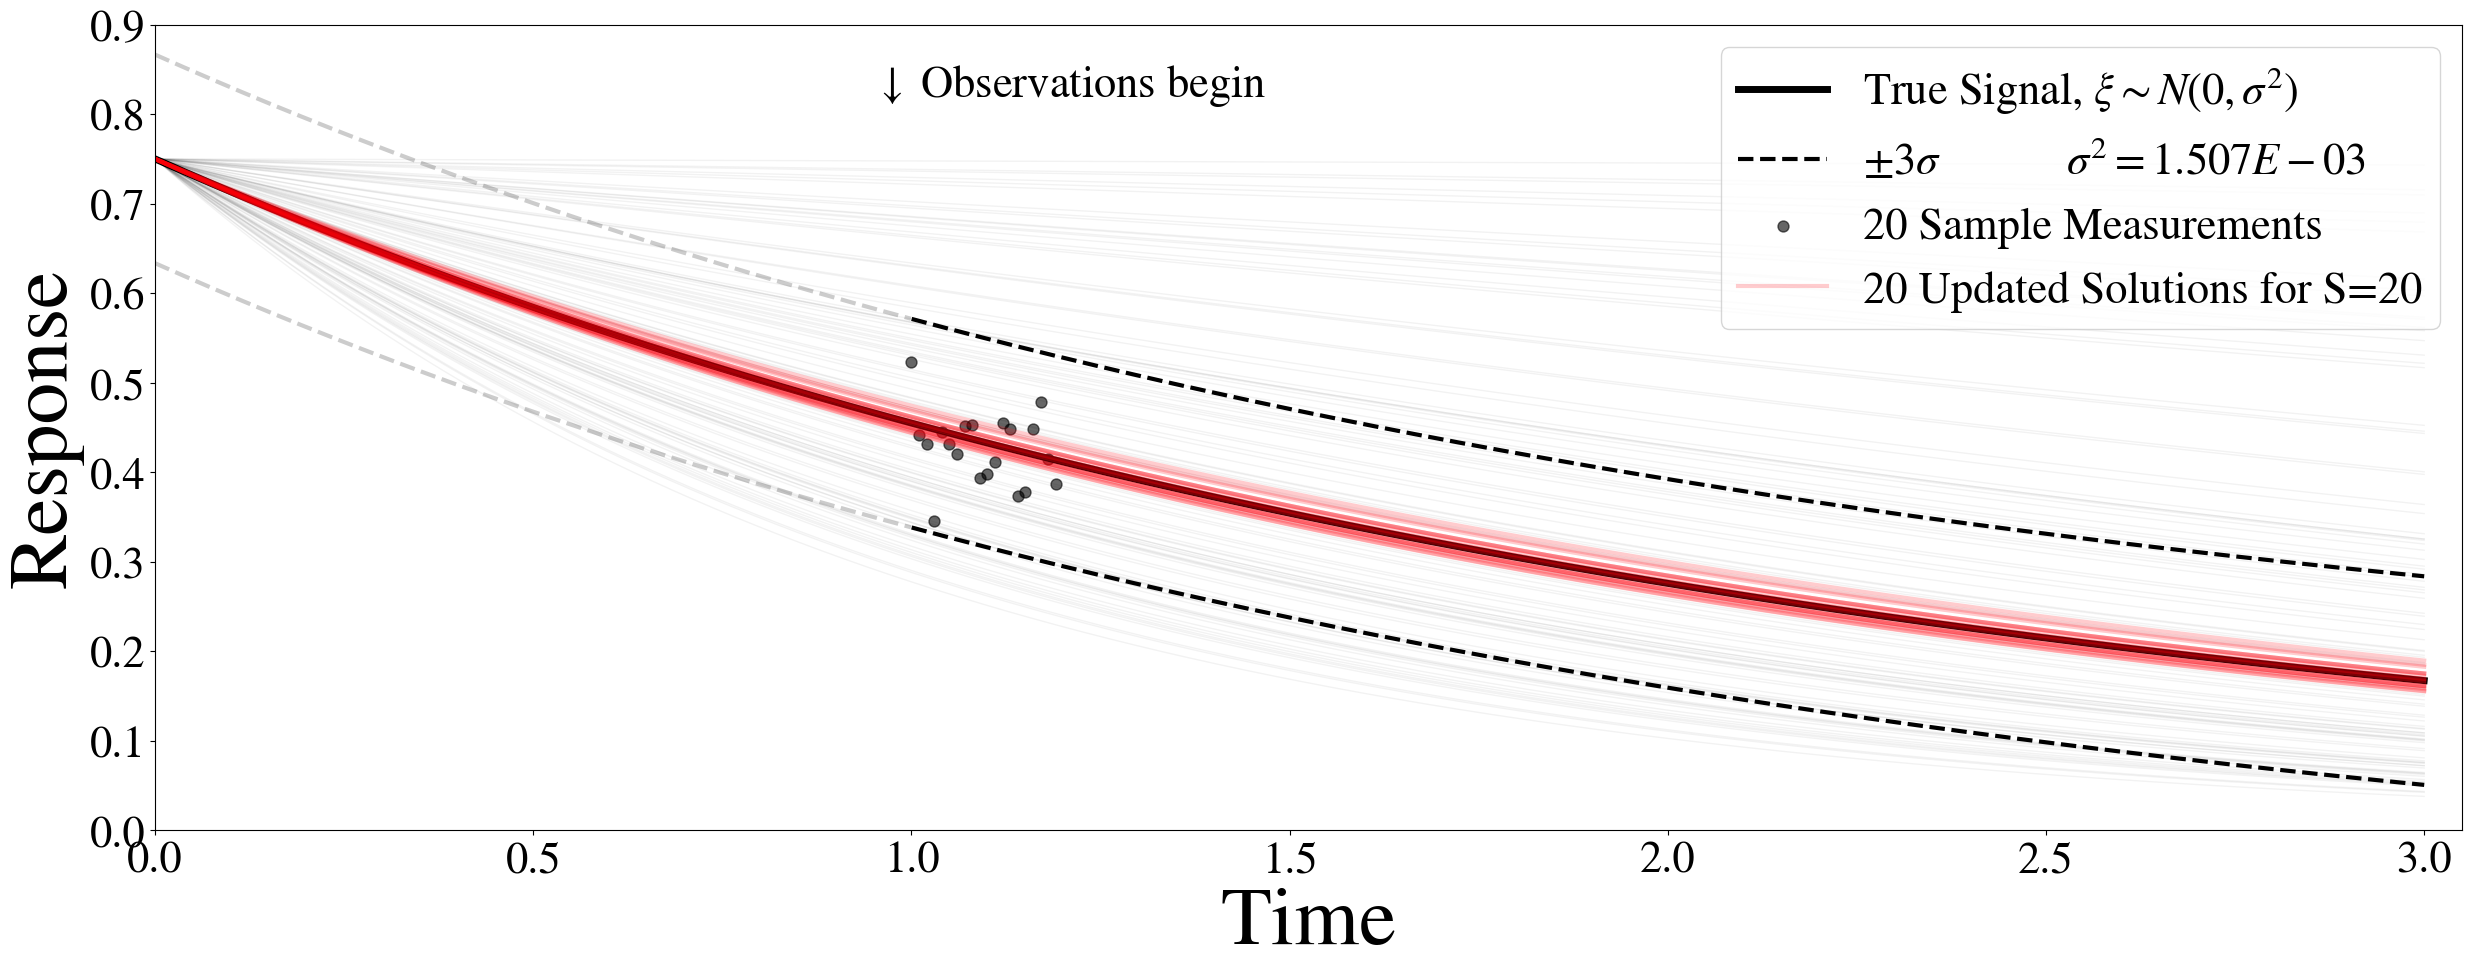
\includegraphics[width=\linewidth]{figures/ode/ode_20_reference_solution}
  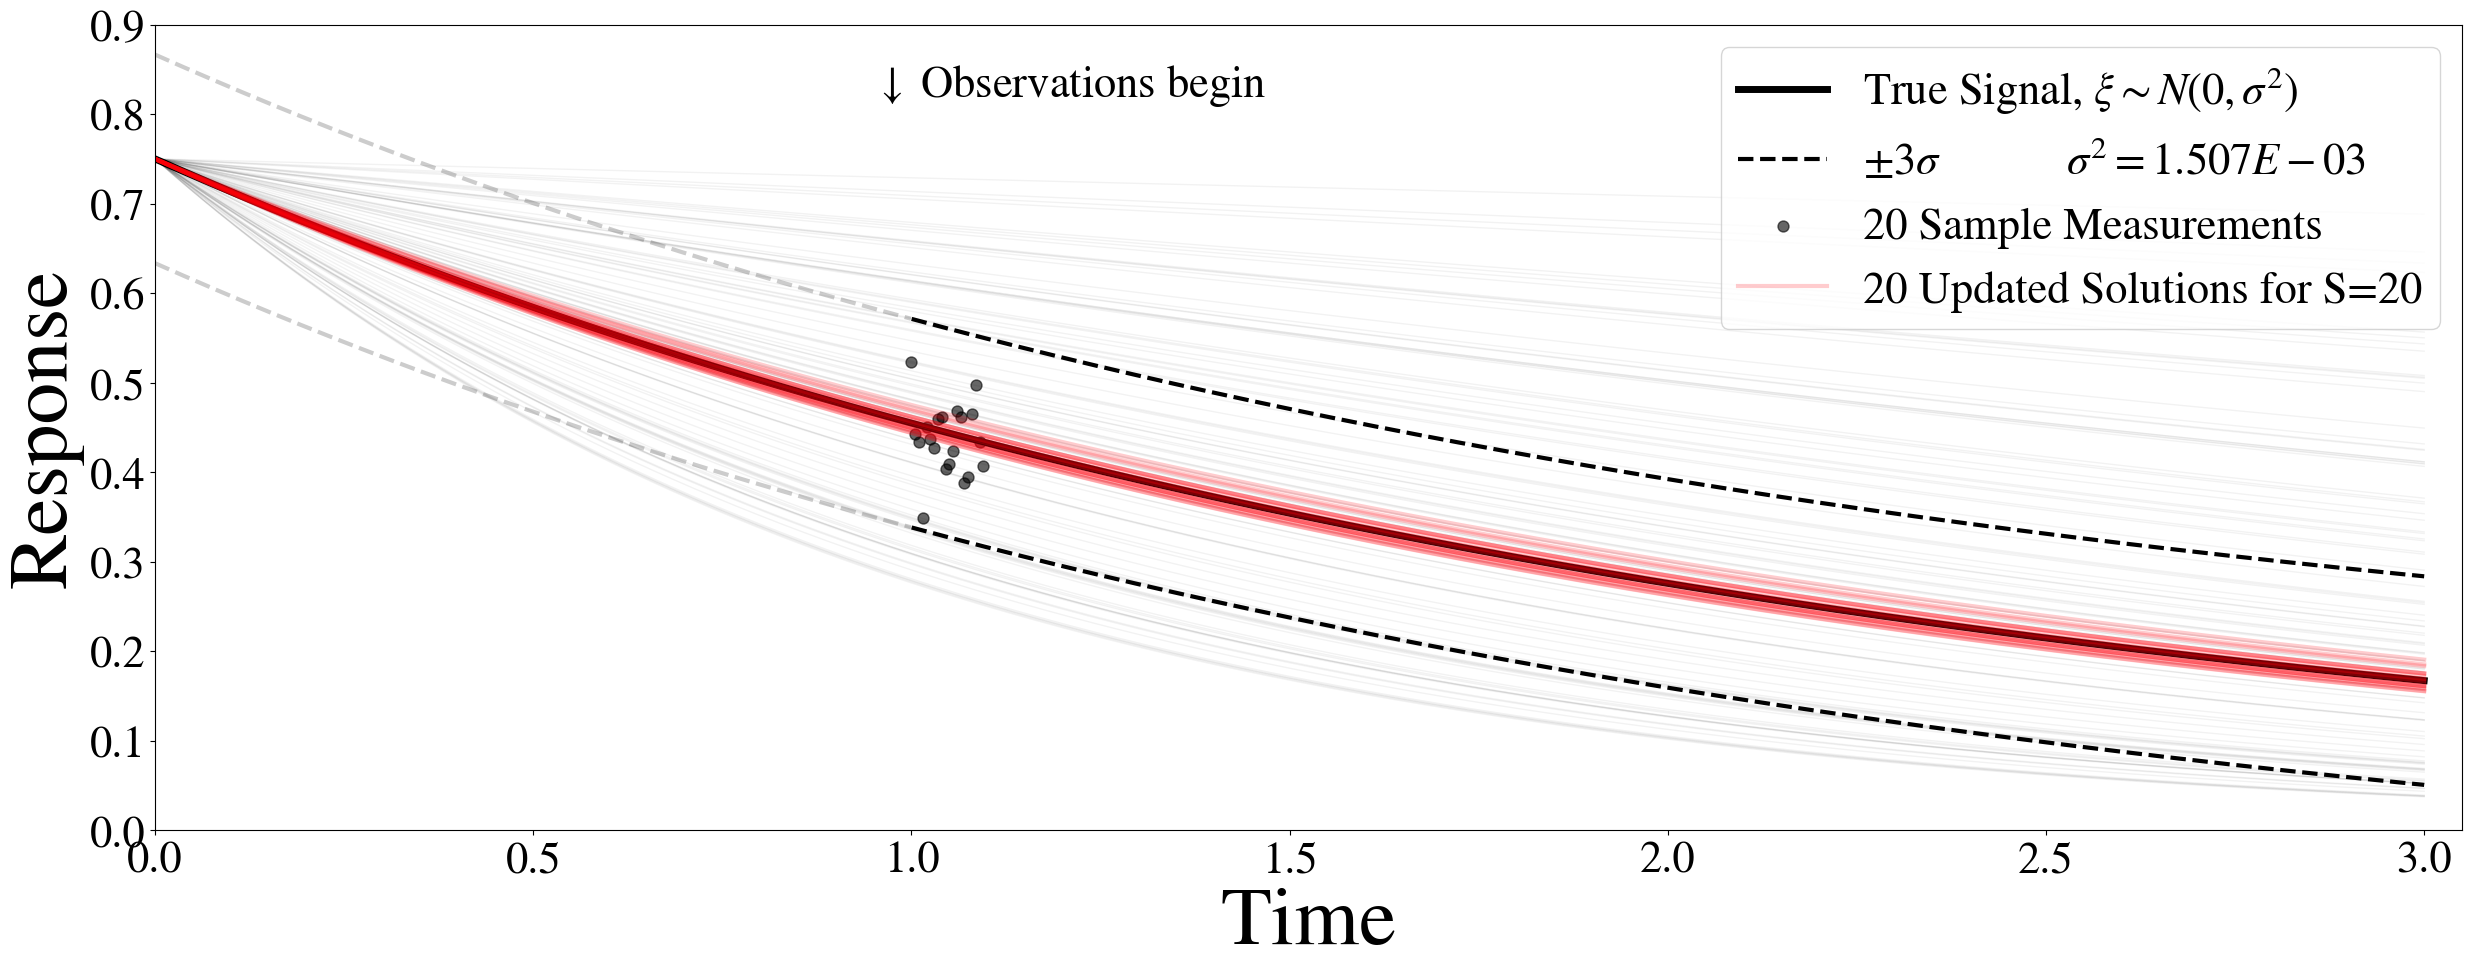
\includegraphics[width=\linewidth]{figures/ode/ode-alt_20_reference_solution}
  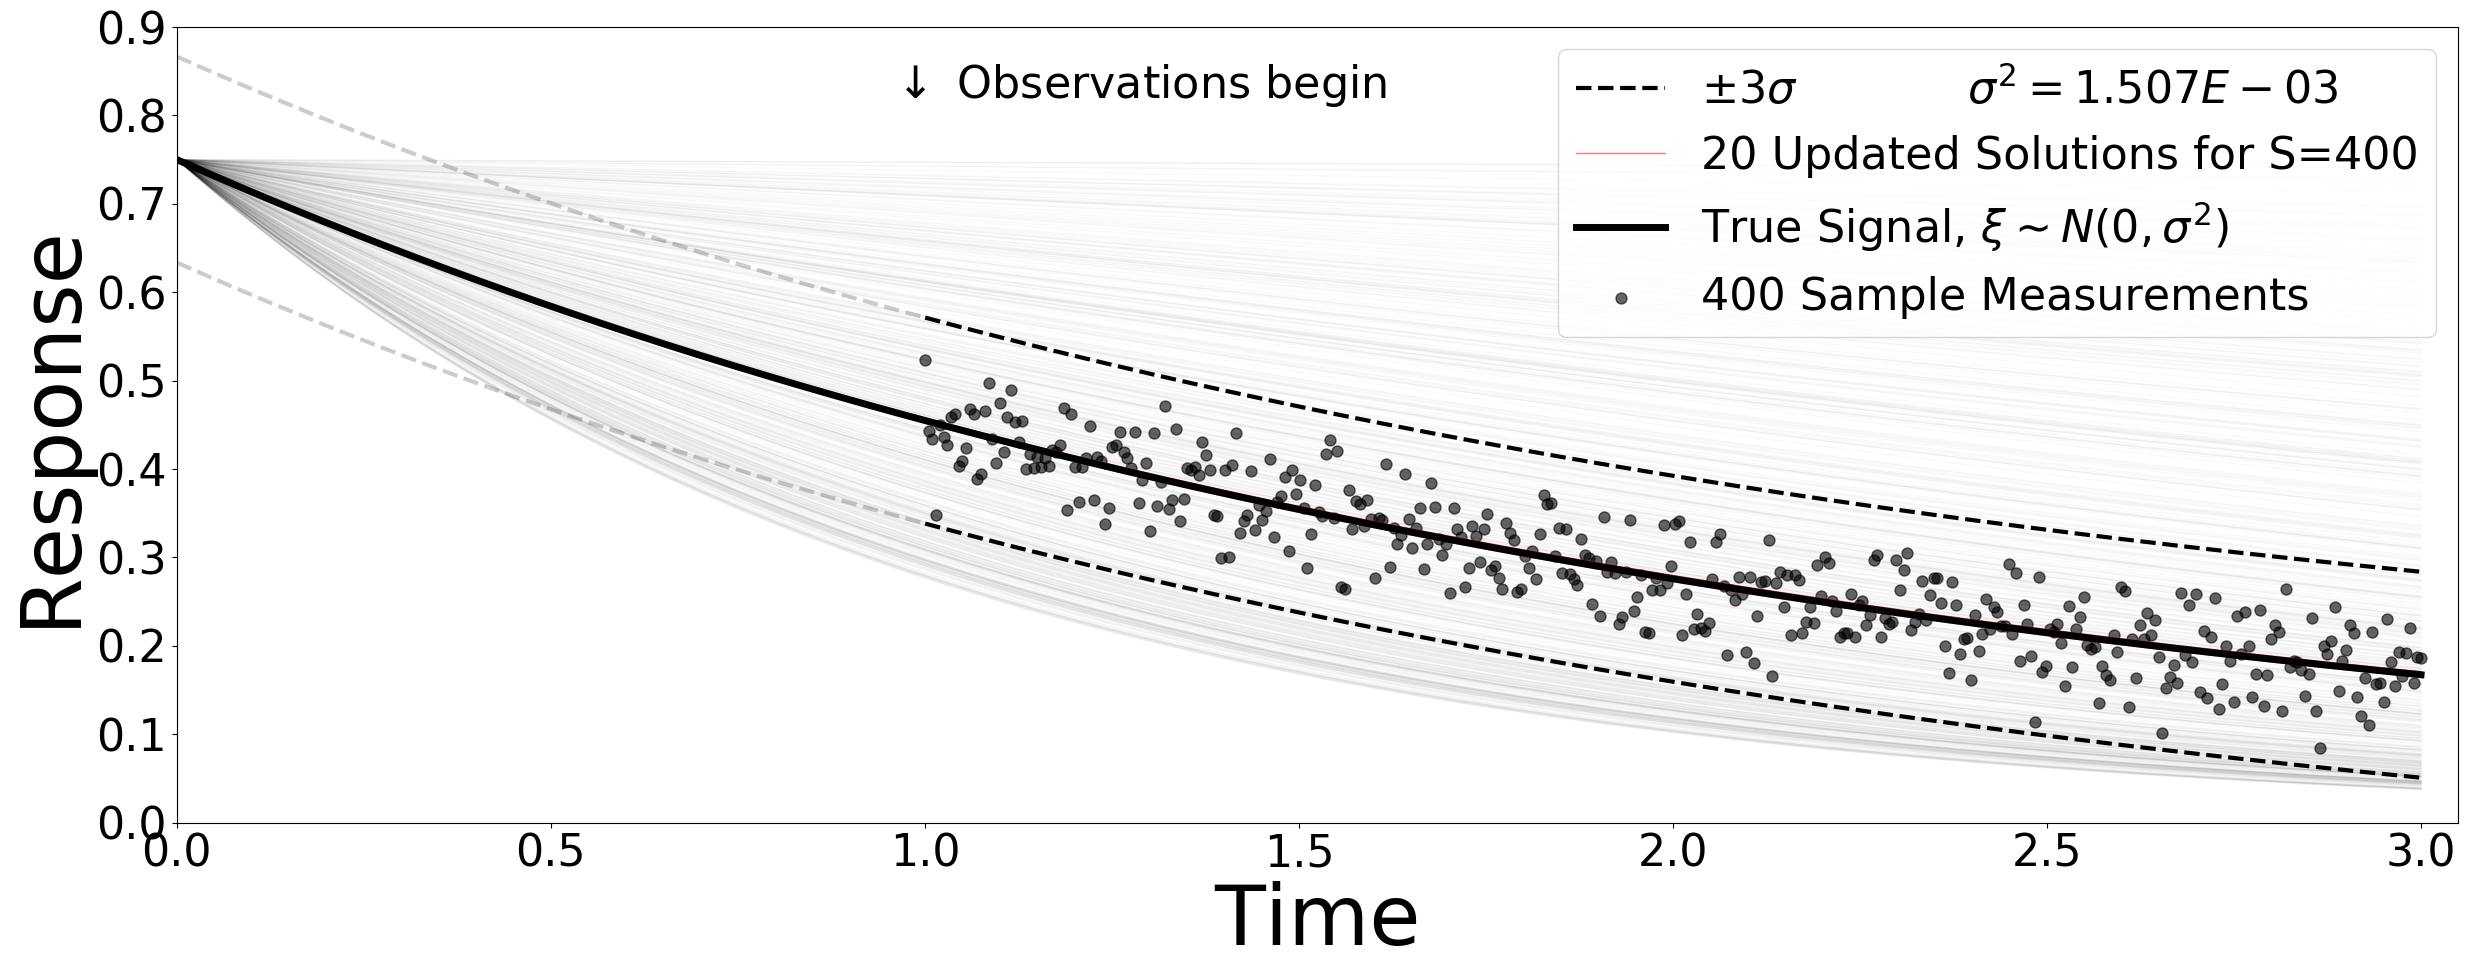
\includegraphics[width=\linewidth]{figures/ode/ode-alt_400_reference_solution}
  \caption{The associated signals for the measurement equipment that operates at twice the frequency.
  The true signal is well-recovered.
  (Top): First twenty measurements used to solve the original problem.
  (Middle): First twenty measurements used to solve the alternative problem.
  (Bottom): The entire value $\param_i$ ($1\leq i \leq N$), in the sampled parameter set.
  }
  \label{fig:ode-alt-reference}
\end{figure}

To quantify accuracy and stability of the MUD solutions, we solve the problem for the same choices of $S$ as the original problem (with the addition of $S=400$).
We show the resulting error plots for convergence in the right half of Figures~\ref{fig:ode-convergence-obs}, juxtaposed against the original experimental design with $100$Hz equipment.

\begin{figure}[htbp]
  \centering
  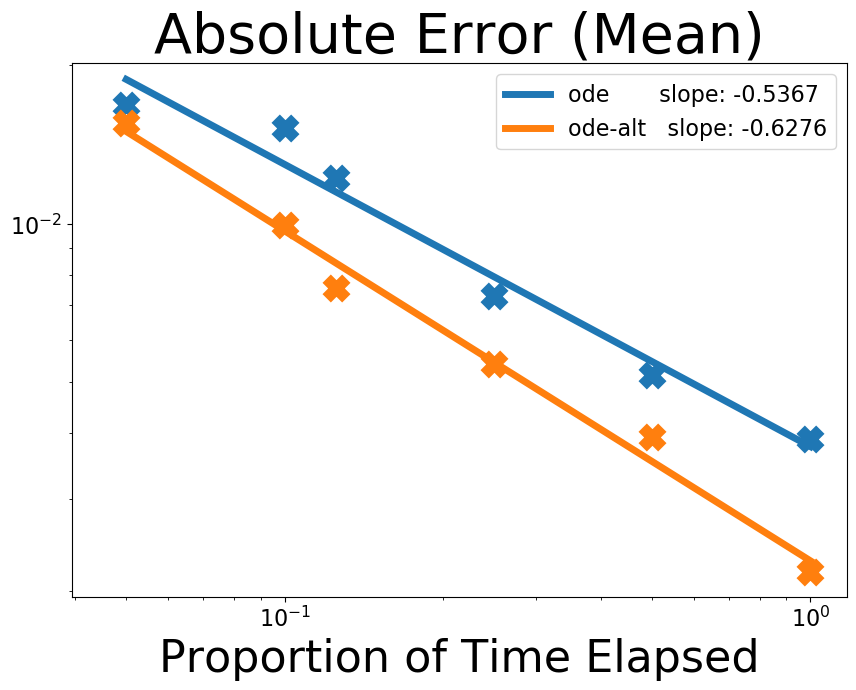
\includegraphics[width=0.475\linewidth]{figures/ode/ode_convergence_mud_obs_mean}
  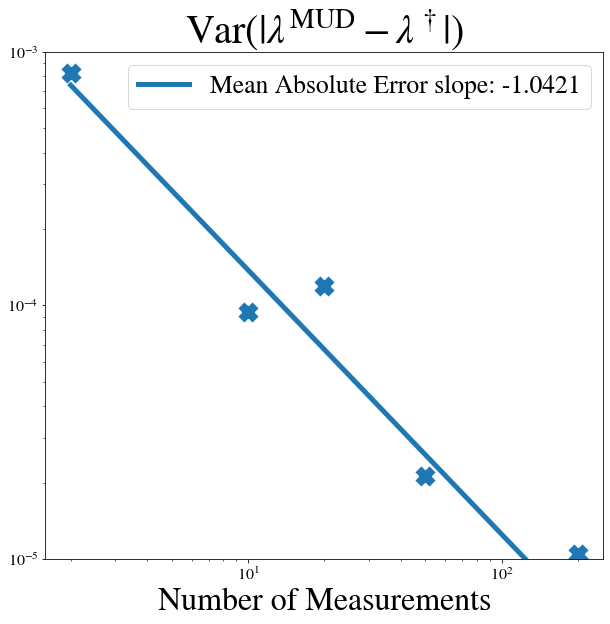
\includegraphics[width=0.425\linewidth]{figures/ode/ode_convergence_mud_obs_var}

  \caption{Convergence of the MUD point given $N=1E4$ model evaluations for increasing numbers of observations for randomly placed sensors.
  Convergence rates are estimated using first-order linear regressions in $\text{log}_{10}$-space.
  $100$Hz equipment demonstrates a reduction of uncertainty and improvement in precision as $S$ increases towards $200$.
  We observe the same rates of convergence for the alternative equipment and note the (slightly) lower overall error for equal numbers of measurements ($S=200$ corresponding to $t\in (1,2)$ in this formulation).
  }
  \label{fig:ode-convergence-obs}
\end{figure}

The convergence rates are similar (shown in the legend of \ref{fig:ode-convergence-obs}), and reduction in uncertainty is almost negligible at a given $S$.
However, we note that in the alternative setup, for an equal number of measurements, the time elapsed is half of that in the original due to the different equipment being used.
To this end, we estimate convergence rates with respect to the time elapsed in the experiment rather than number of measurements used, and notice that the alternative setup (orange) exhibits much lower error at a given point of time.
This implies that we can achieve similar results with a shorter observational window by using equipment that allows for faster observations.



%%%%%%%%%%%%%%%%%%%%%%%%%%%%%%%%%%%%%%%%%%%%%%%%%%%%%%%%%%%%%%%%%%%%
\FloatBarrier
%%%%%%%%%%%%%%%%%%%%%%%%%%%%%%%%%%%%%%%%%%%%%%%%%%%%%%%%%%%%%%%%%%%%

\subsubsection{Impact of Equipment Precision}
We expect that a method designed to address parameter estimation would see an improvement in accuracy  if the data is collected with more precise instruments.
To achieve higher precision in the estimate of the MUD point, one can use more precise measurement equipment.
Here we show that this is indeed the case for the time-series example introduced earlier by considering choices of $\tau = 0.1, 0.05, 0.01, \text{ and } 0.005$ for $\mathbb{P}( \abs{\xi} < \tau ) = 99\%$ to select our $\sigma$ in our normal additive noise model.
We sequentially incorporate $S=5, 10, 15, 20, 25, 50, 100, \text{ and } 200$ measurements and study the error in our estimate of $\paramref$.



\begin{figure}[htbp]
  \centering
  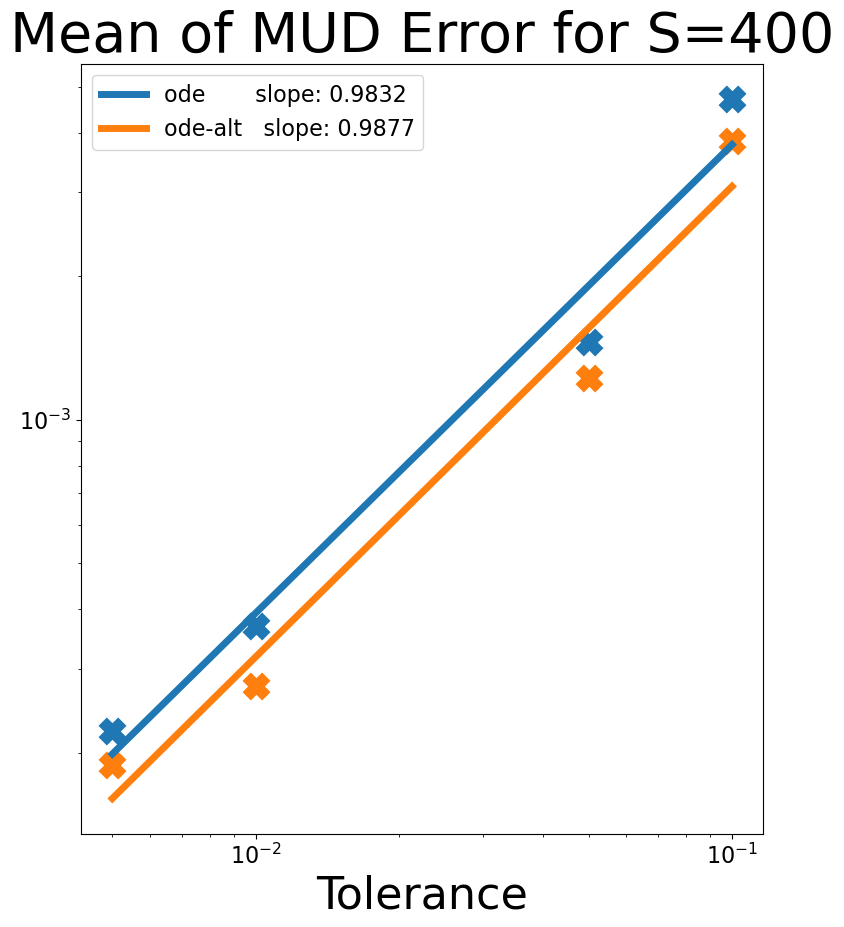
\includegraphics[width=0.475\linewidth]{figures/ode/ode_convergence_mud_std_mean}
  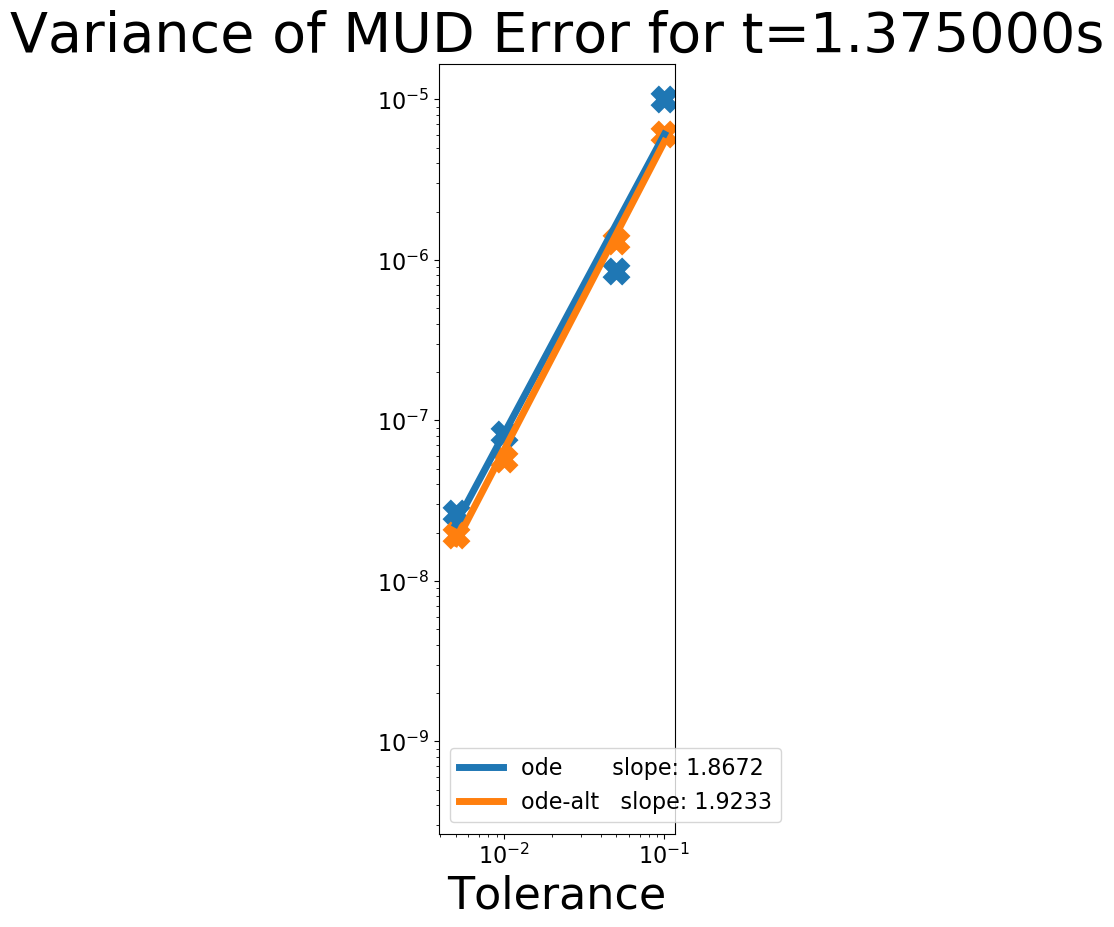
\includegraphics[width=0.425\linewidth]{figures/ode/ode_convergence_mud_std_var}

  \caption{[TK - FIX THE TITLES (manually specified). This is supposed to be at t=1.375]. Convergence of the MUD point given $N=1E4$ model evaluations incorporating measurements at a fixed point in time.
  As more precise measurements are incorporated, the accuracy and precision of the MUD solution improves.
  }
  \label{fig:ode-convergence-std}
\end{figure}

In Figure~\ref{fig:ode-convergence-std}, we study the absolute error's mean and variance as our measurement equipment gets more precise (lower tolerance), for both the $100$Hz (ode) and $200$Hz (ode-alt) variants of sensor.
In the left half of the figure, we find that the convergence rates for the two designs are nearly identical but the equipment which records twice as many measurements has a persistent reduction in error.
The right half shows the convergence in variance of the absolute error, and the vertical displacement between the two designs is visually difficult to distinguish.
However, as evidenced in the legends, the alternative design (faster equipment) exhibits an increase in the rate of convergence from 1.87 to 1.92.

We have shown that the Data--Consistent approach to solving parameter identification problems manages to generalize to problems involving time-series data from a single Quantity of Interest.
We now turn our attention to an example where instead of temporal measurements, we incorporate spatial ones to solve another parameter identification problem.

%%%%%%%%%%%%%%%%%%%%%%%%%%%%%%%%%%%%%%%%%%%%%%%%%%%%%%%%%%%%%%%%%%%%
%%%%%%%%%%%%%%%%%%%%%%%%%%%%%%%%%%%%%%%%%%%%%%%%%%%%%%%%%%%%%%%%%%%%
\FloatBarrier
%%%%%%%%%%%%%%%%%%%%%%%%%%%%%%%%%%%%%%%%%%%%%%%%%%%%%%%%%%%%%%%%%%%%
%%%%%%%%%%%%%%%%%%%%%%%%%%%%%%%%%%%%%%%%%%%%%%%%%%%%%%%%%%%%%%%%%%%%
\subsection{Elliptic PDE Example}\label{subsec:pde-example}

Consider the following Poisson problem defined on a unit domain $\Omega$:
\begin{equation}\label{eq:pde-equation}
\begin{cases}
\hfill -\nabla \cdot \nabla u &= f \quad\text{on } \Omega \\
\hfill u &= 0 \quad\text{ on } \Gamma_T \cup \Gamma_B \\
\hfill \frac{\partial u}{\partial \mathbf{n}} &= g(x,\param) \quad\text{ on } \Gamma_L \\
\hfill \frac{\partial u}{\partial \mathbf{n}} &= 0 \quad\text{ on } \Gamma_R
\end{cases}
\end{equation}
where $(x_1, x_2) \in \Omega = (0,1)^2$, $\Gamma_T$ is the top, $\Gamma_B$ is the bottom, $\Gamma_L$ and $\Gamma_R$ left and right, respectively.
$\frac{\partial u}{\partial \mathbf{n}}$ denotes the outward normal direction.

\begin{figure}
\centering
  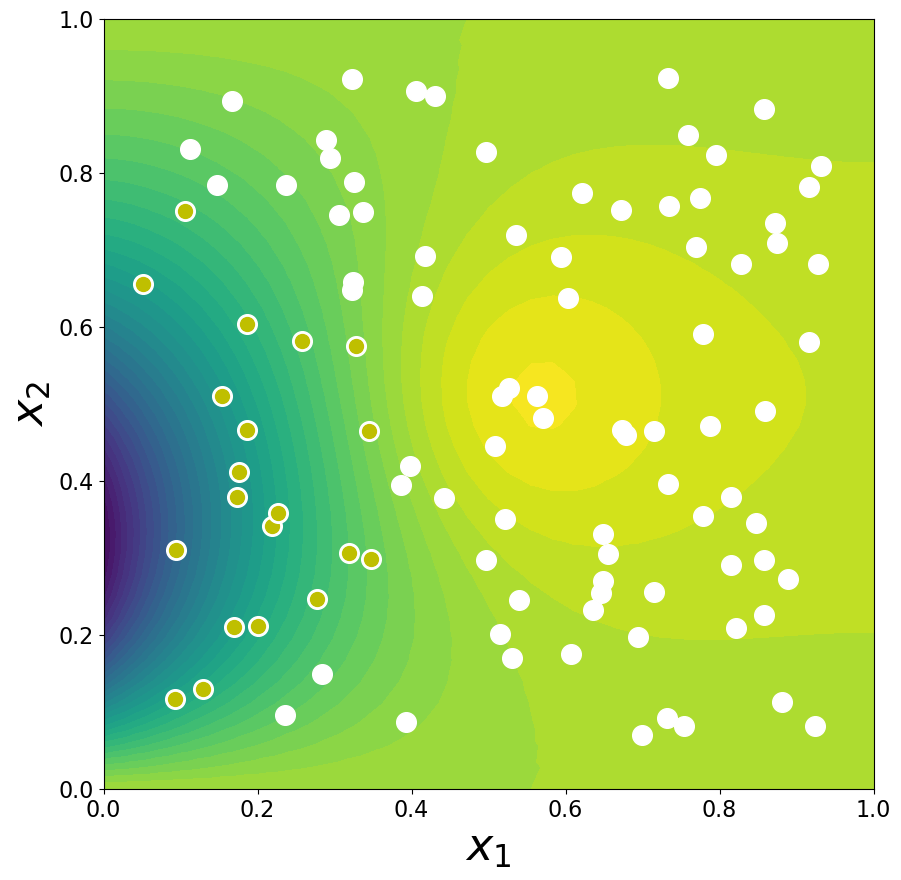
\includegraphics[width=0.475\linewidth]{figures/pde/pde_reference_solution}
  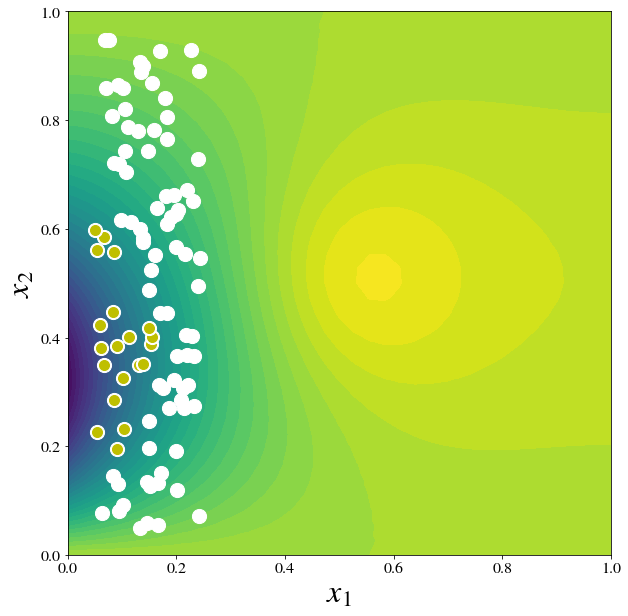
\includegraphics[width=0.475\linewidth]{figures/pde/pde-alt_reference_solution}
\caption{The function response surface for $u$ solving \eqref{eq:pde-equation} with $S=100$ measurement locations highlighted in white.
The twenty most sensitive locations are highlighted in yellow.
(Top): Uninformed sensor placement, where the most sensitive points  appear to cluster around the center of the  left boundary.
This observation is used to inform a better placement.
(Bottom): An alternative random arrangement of $S=100$ measurement locations.
}
\label{fig:pde-ref-solution}
\end{figure}
We select $g=\param \sin(\pi x_2)$, and show the response surface for our given choice of $\param = 3$ in Figure~\ref{fig:pde-ref-solution}.
Our initial density is chosen to be uniform over the interval $\Lambda = (1,5)$.
$f$ is chosen to be $10\exp\{-\frac{(x_1-0.5)^2 + (x_2 - 0.5)^2}{0.02}\}$


We are interested in demonstrating the impact of incorporating more measurements on our ability to estimate $\paramref$.
This poses a problem for this particular experimental design since it will heavily rely on the way in which the sensor grid is indexed.
One could place a regular grid of sensors in the interior of $\Omega$ to simulate a sensor array of some sort.
However, observe that the response surfaces shown in Figure~\ref{fig:pde-ref-solution} exhibit vertical symmetry about the line $x_2=0.5$ (as a result of our choice of $g$).


For example, if the first half of indexed sensors corresponded to the bottom half of $\Omega$, the incorporation of the second half will be equivalent to having repeated observations.
Moreover, since the left-side of $\Omega$ is more sensitive to changes in $\param$ than the right, indexing in a serpentine manner will lead to sharper declines in uncertainty whenever a sensor from a different row gets incorporated.
To avoid these problems, we instead simulate the sensors as being placed randomly in the interior so that index-dependence becomes irrelevant and  probability theory ensures the lack of truly redundant measurement locations.

%%%%%%%%%%%%%%%%%%%%%%%%%%%%%%%%%%%%%%%%%%%%%%%%%%%%%%%%%%%%%%%%%%%%
%%%%%%%%%%%%%%%%%%%%%%%%%%%%%%%%%%%%%%%%%%%%%%%%%%%%%%%%%%%%%%%%%%%%
\subsubsection{Uninformed Sensor Placement}

Returning to the PDE example from [TK - ch4 section 6], recall that there we had the following experimental setup, which we use here as well:
We consider a selection of $S=1000$ measurement locations in the interior of the response surface chosen by sampling a uniform density over the set $(0.05, 0.95)^2 \subset \Omega$.
In Figure~\ref{fig:pde-sensitivity}, we plot the data generated by each simulated sensor location, and observe that some measurements are more sensitive than others.
The majority of measurements exhibit almost no sensitivity to changes in $\param$, visually represented by the density of nearly horizontal lines.
However, some of the sensors have steep slopes, which indicates higher sensitivity to changes in $\param$.


\begin{figure}
\centering
  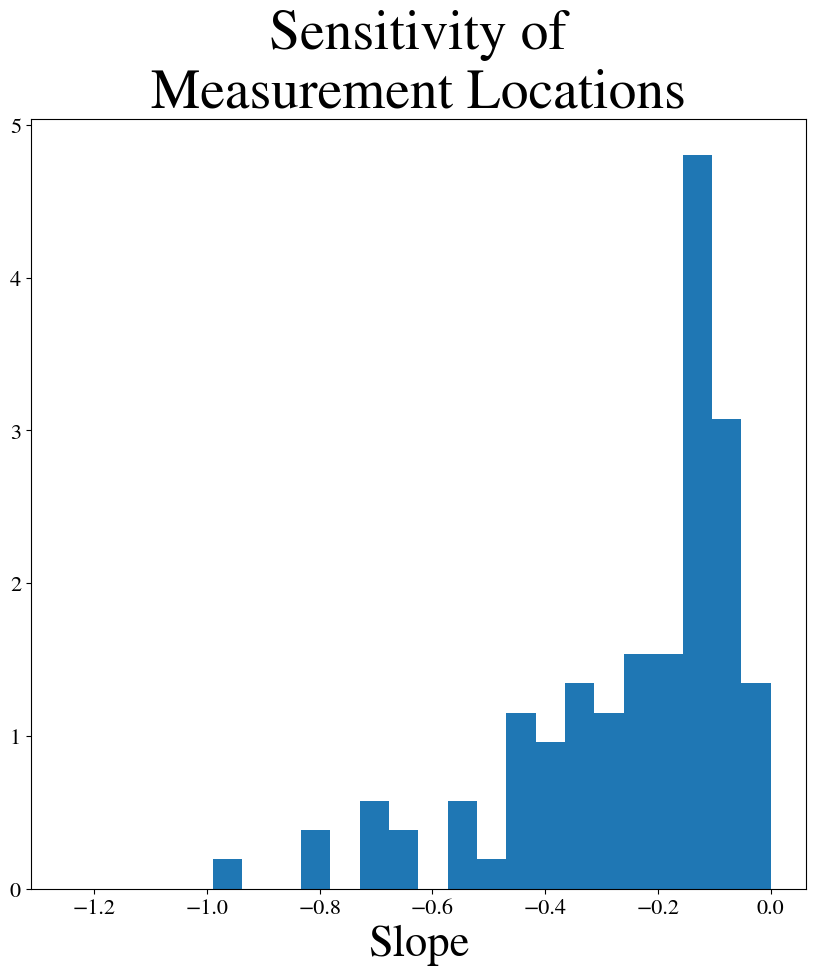
\includegraphics[width=0.35\linewidth]{figures/pde/pde_sensitivity_qoi}
  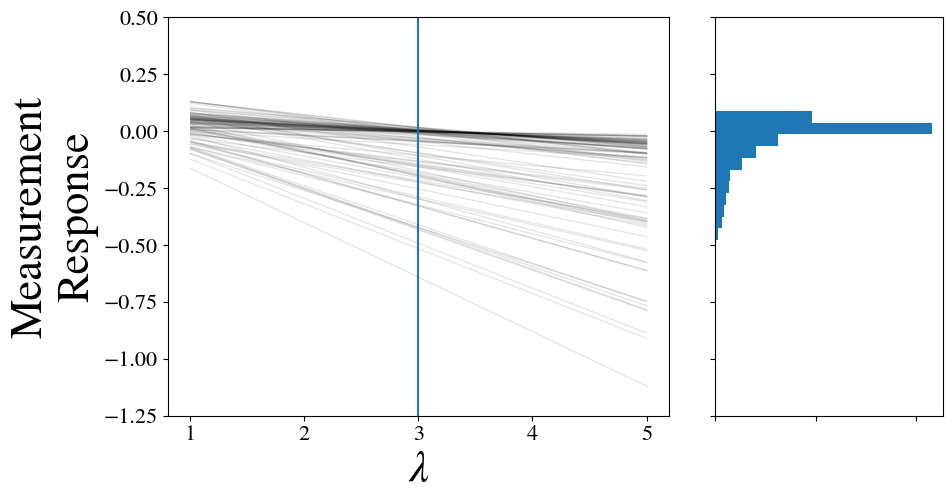
\includegraphics[width=0.6\linewidth]{figures/pde/pde_qoi_response}
  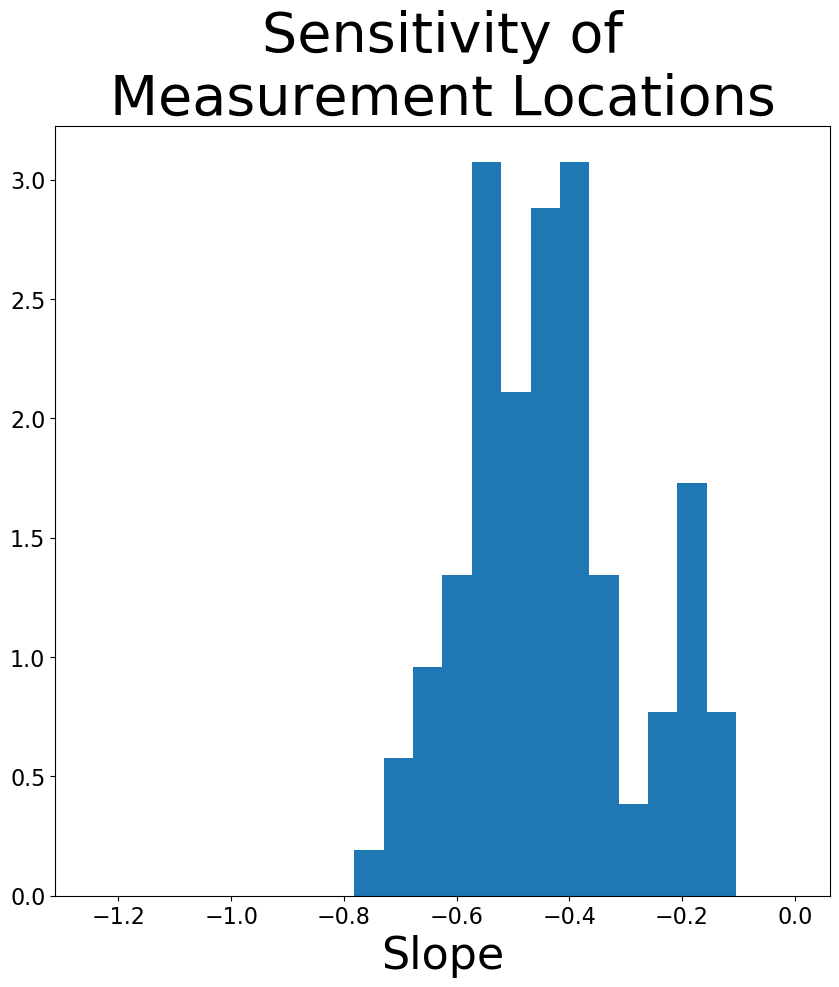
\includegraphics[width=0.35\linewidth]{figures/pde/pde-alt_sensitivity_qoi}
  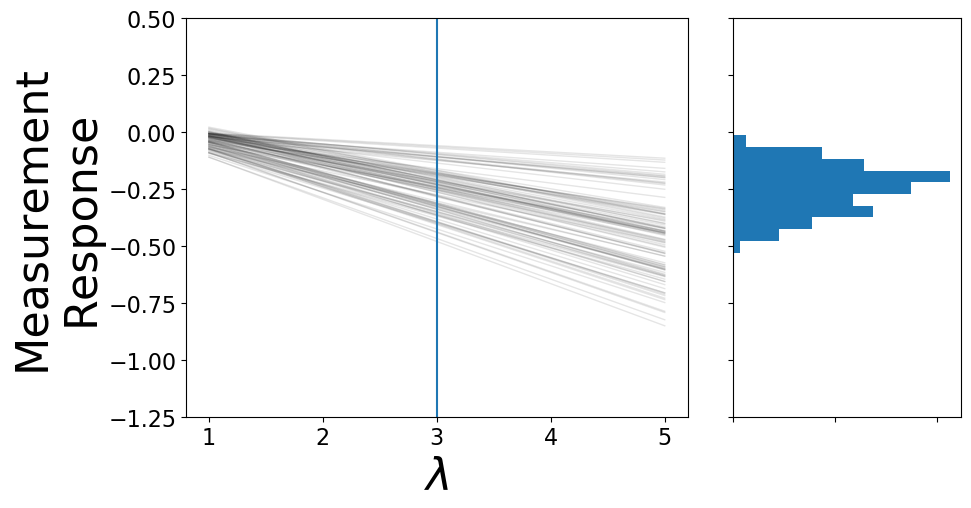
\includegraphics[width=0.6\linewidth]{figures/pde/pde-alt_qoi_response}
  \caption{Sensitivity of measurements as a function of $\param$, the scaling for the left boundary condition function.
  We plot the values of the response surface evaluated at all $S=1000$ random measurement locations.
  Since the response at each measurement location is linear with respect to $\param$, we can compute the slopes for all $S=1000$ sensors and show the associated histogram (left).
  (Top): Uninformed sensor placement. Observe that most locations are insensitive to changes in $\param$.
  (Bottom): Informed sensor placement. The informed sensors have much less variability in their respective sensitivities.
  }
\label{fig:pde-sensitivity}
\end{figure}



We are interested in knowing how the uncertainty around the parameter estimate (the MUD point) changes as we incorporate more (noisy) data.
Consider the plots in the left-half of Figure~\ref{fig:pde-convergence-obs}, which demonstrates the impact of increasing $S$ on our ability to resolve $\paramref$.
To generate convergence plots, we use all thousand available measurements but solve the problem repeatedly for $S = 5, 10, 15, 20, 25, 50, 100, 250, 500, \text{ and } 1000$.
For visual clarity, we plot the first hundred sensors on plots which do not show convergence.

\begin{figure}
  \centering
  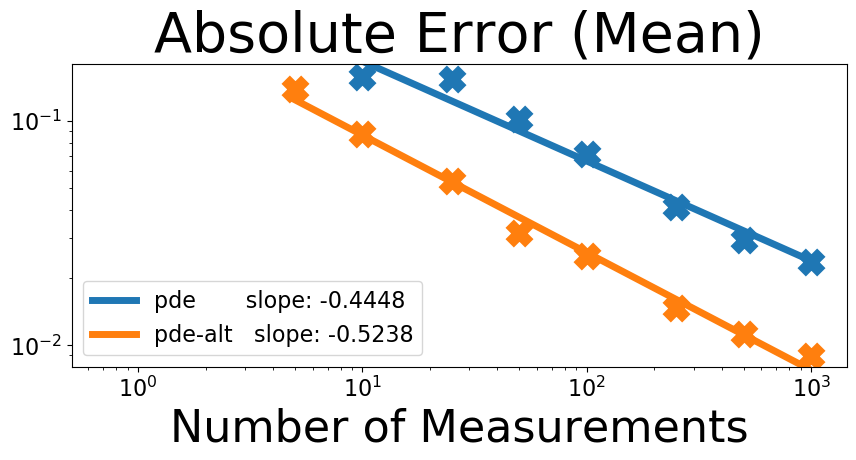
\includegraphics[width=0.475\linewidth]{figures/pde/pde_convergence_mud_obs_mean}
  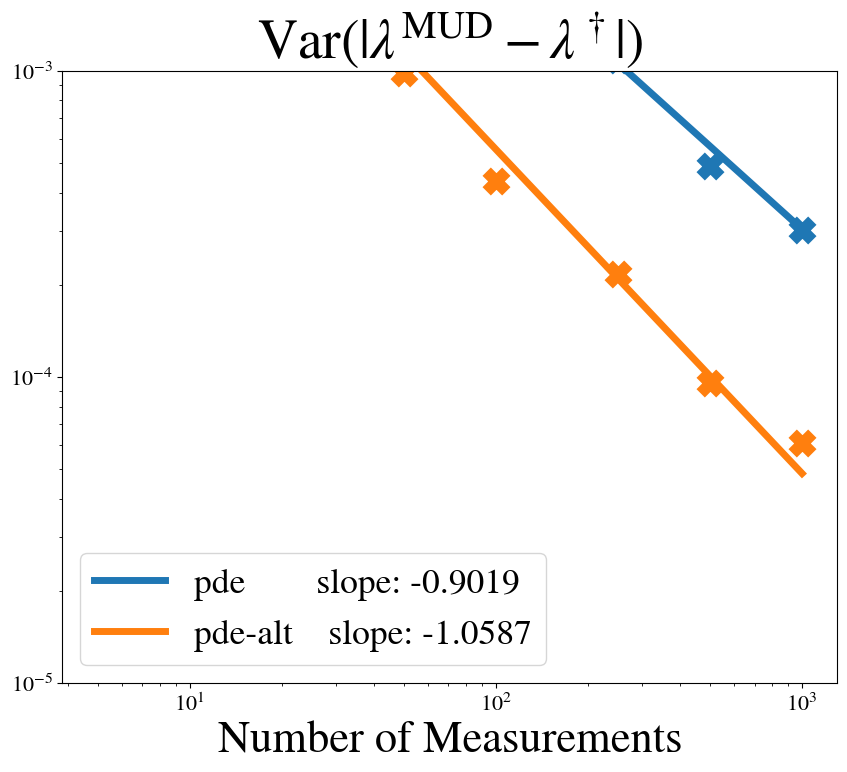
\includegraphics[width=0.475\linewidth]{figures/pde/pde_convergence_mud_obs_var}
  \caption{Convergence of the MUD point (given $N=1E3$ model evaluations) for increasing numbers of observations for randomly placed sensors.
  We observe similar rates of convergence for both arrangements of measurement locations, with a marked improvement in both accuracy and precision when an informed placement is used.
  }
  \label{fig:pde-convergence-obs}
\end{figure}


Similar to \ref{fig:ode-convergence-std}, we demonstrate that using more sensitive measurement equipment improves the estimation of the MUD point.
Again we consider choices of standard deviation associated with $\tau = 0.1, 0.05, 0.01, \text{ and } 0.005$ for $\mathbb{P}( \abs{\xi} < \tau ) = 99\%$.
In Figure~\ref{fig:pde-convergence-std}, we study the impact of more precise measurement equipment on the absolute error's mean and variance.

\begin{figure}[htbp]
  \centering
  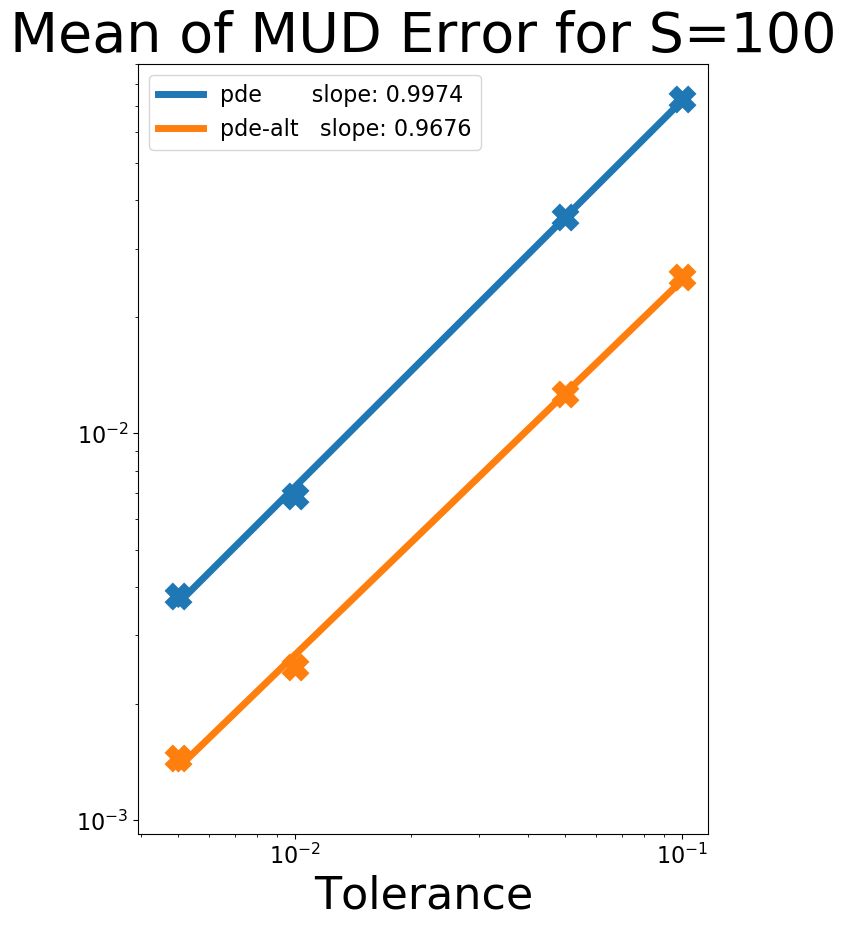
\includegraphics[width=0.475\linewidth]{figures/pde/pde_convergence_mud_std_mean}
  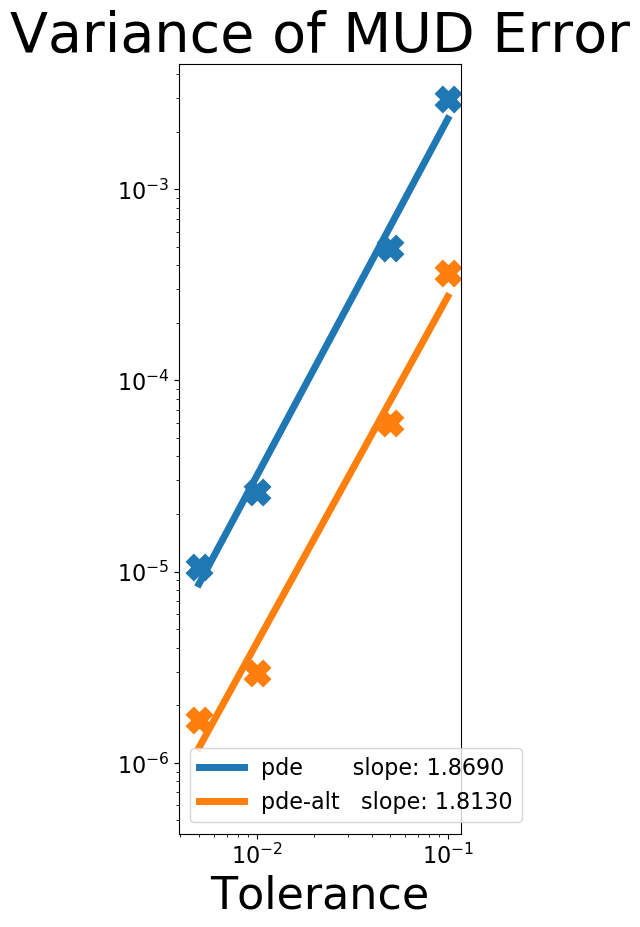
\includegraphics[width=0.475\linewidth]{figures/pde/pde_convergence_mud_std_var}
  \caption{Convergence of the MUD point given $N=1E4$ model evaluations for different measurement precisions for randomly placed sensors, incorporating $S=100$ measurements.
  We note that the convergence rates are the same but the overall accuracy and precision improve when sensors are placed in regions of $u$ that exhibit higher sensitivity to changes in $\param$.
  }
  \label{fig:pde-convergence-std}
\end{figure}


These results demonstrate that even randomly placed sensors in the interior of $\Omega$ are suitable for parameter estimation.
Figure~\ref{fig:pde-ref-solution} highlights the twenty most sensitive sensors, which appear by the left boundary of the domain; choosing sensors more carefully using this information could lead to improved accuracy with fewer sensors.
We now demonstrate how such an observation can be incorporated into our experimental design choices.


\subsubsection{Informed Sensor Placement}
Instead of placing sensors throughout the square interior of $\Omega$ given by $(0.05, 0.95)^2$, we briefly consider how the convergence results would change if the subdomain for sensors was better chosen to be near the left boundary.
Furthermore, the response surface exhibits horizontal symmetry, so we restrict locations to the bottom half of $\Omega$.
We perform the same experiment for sensors placed in $(0.05, 0.25)\times(0.05, 0.5)$ and show the results in

We demonstrate the sensitivities of each sensor in the right half of Figure~\ref{fig:pde-sensitivity}, and note that there are fewer sensors which exhibit low sensitivity to changes in $\paramref$.
It appears in the right half of Figure~\ref{fig:pde-convergence-obs}, that two decimal places of accuracy can be achieved with approximately $250$ samples instead of the $1000$ required in the left-half.


\subsection{Concluding Remarks for Examples}

These examples demonstrate that Data--Consistent Inversion can be used for parameter identification as a viable alternative to existing methods.
The problems in this section have involved one-dimensional output spaces, and solely demonstrate one method by which measurements can be transformed into a QoI map.
The problems have also involved one-dimensional parameter spaces, limiting the useful dimension of the QoI map we construct.
We address these concerns in the next section by extending the previous (PDE) example to a vector-valued analogue with the original experimental design for collecting measurements in $(0.05, 0.95)^2$.

We point out that in the framework of collapsing available observations of data leaves the output space as scalar-valued.
As the number of parameters grows, this output dimension effectively stays fixed.
This is particularly when the DCI approach becomes advantageous over other methods as it is less sensitive to mistakes in modeling assumptions than other methods for solving inverse problems.
One can incorporate a much wider variety of prior beliefs about the relative likelihoods of parameters before data is collected without compromising predictive error.
The DCI approach guarantees that the functional defined (for us, the weighted mean error) will remain accurate in spite of any encoded assumptions that are somehow at odds with data that is subsequently collected.
